\chapter{Głębokie sieci neuronowe}
\label{roz2}

\hspace{0.4cm}
Głębokie uczenie jest częścią dziedziny uczenia maszynowego, rozwijającą się poprzez wykorzystanie wielowarstwowych sieci neuronowych. Wiele warstw przetwarza informacje tworząc hierarchię cech zaczynając od najprostszych do coraz bardziej abstrakcyjnych koncepcji, np. graficznych. Początkowe warstwy starają się nauczyć określonych struktur danych, aby kolejne korzystając z nich mogły rozpoznawać bardziej złożone i skomplikowane obiekty, często złożone z elementów zaprezentowanych poprzednio.
Ze względu na swoje działanie sieci te znalazły wiele zastosowań w różnych zadaniach z~zakresu przetwarzania mediów, czy w systemach decyzyjnych i~rekomendacyjnych \cite{OsowskiSieci}.

Schemat \ref{fig:schematsieci} w uproszczony sposób przedstawia warstwową organizację neuronów i ich połączenia między sobą. Można wyróżnić trzy podstawowe warstwy

\begin{itemize}
    \item[--] \textbf{warstwę wejściową}, do której dostarczane są dane wejściowe,
    \item[--] \textbf{jedna lub więcej warstw ukrytych}, które przetwarzają otrzymaną informację,
    \item[--] \textbf{warstwa wyjściowa}, przechowująca wyniki.
\end{itemize}

\begin{figure}[H]
    \centering
    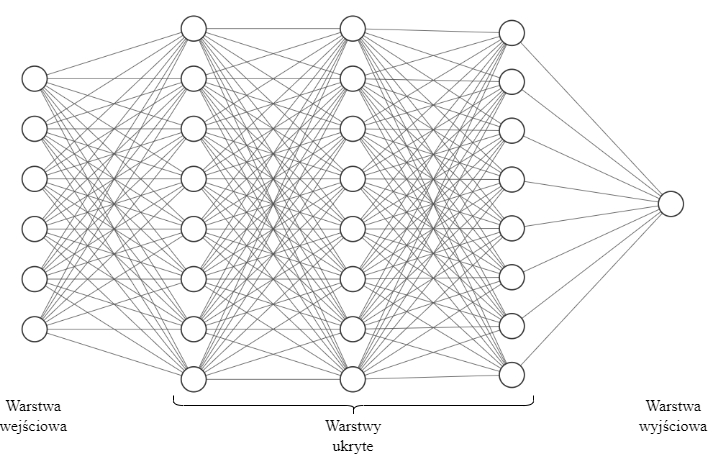
\includegraphics[width=0.9\linewidth]{Obrazy/Rozdzial02/schematsieci.png}
    \caption{Uproszczony schemat głębokiej sieci neuronowej.}
    \label{fig:schematsieci}
\end{figure}


Głębokością sieci neuronowej nazywana jest liczba warstw jej modelu danych. Mimo, iż nie została wyznaczona bezwzględna granica, ile warstw powinna mieć sieć aby uznać ją za głęboką, przyjęło się, że jest nią każdy system złożony z więcej niż dwóch warstw ukrytych.

\section{Konwolucyjne sieci neuronowe}
\label{roz2.1}

\hspace{0.4cm}
Typem jednokierunkowych sieci w uczeniu głębokim są sieci konwolucyjne (CNN). Ich nazwa pochodzi od operacji konwolucji tj. połączeniu dwóch funkcji

\begin{equation}
    y(n) = x(n) \ast w(n) = \sum_{i=-\infty}^\infty x(i)w(n-1) = \sum_{i=-\inty}^\infty x(n-i)w(i)
\end{equation}

\noindent
gdzie argumenty $x(n)$ i $w(n)$ oznaczają odpowiednio wejście i jądro przekształcenia. Wynik $y$~określa odwzorowanie cech.  \cite{DeepLearning} 


Sieci konwolucyjne wykorzystywane są najczęściej do zadań związanych z przetwarzaniem obrazów, dlatego operacja splotu musi zostać wykonana w więcej niż jednym wymiarze. Wtedy tablica danych wejściowych reprezentowana jest jako dwuwymiarowy obraz \textbf{I} z dwuwymiarowym jądrem \textbf{K}

\begin{equation}
    \textbf{Y}(i,j) = \textbf{I}(i,j) \ast \textbf{K}(i,j) = \sum_m \sum_n \textbf{I}(m,n)\textbf{K}(i-m,j-n) = \sum_m \sum_n \textbf{I}(i-m,j-n)\textbf{K}(m,n)
\end{equation}

W przeciwieństwie do niektórych architektur sieci, które realizują wszystkie możliwe połączenia międzywarstwowe, w sieciach konwolucyjnych neurony kolejnych warstw łączą się jedynie z pewnym określonym obszarem neuronów z poprzedniej. Taki sposób połączeń przyspiesza znacznie proces treningu, pomimo możliwie dużej ilości wykorzystywanych parametrów. 

Kolejną zaletą jest nauka lokalnych wzorców, co ponownie odróżnia je od pozostałych sieci głębokich. Dzięki tej własności sieci są w stanie rozpoznać wyuczony wzorzec niezależnie od miejsca jego występowania, bez konieczności uczenia się go na nowo. Dodatkowo sieci mogą uczyć się wzorców w sposób hierarchiczny tj. każda kolejna warstwa konwolucyjna uczy się lokalnych wzorców, które mogą się składać z elementów rozpoznanych w poprzednich etapach \cite{Python}.

\section{Budowa sieci}
\label{roz2.2}

\hspace{0.4cm}
Standardowa sieć konwolucyjna składa się z kombinacji kilku typów warstw, spełniających odpowiednią rolę w całym układzie.

\begin{figure}[H]
    \centering
    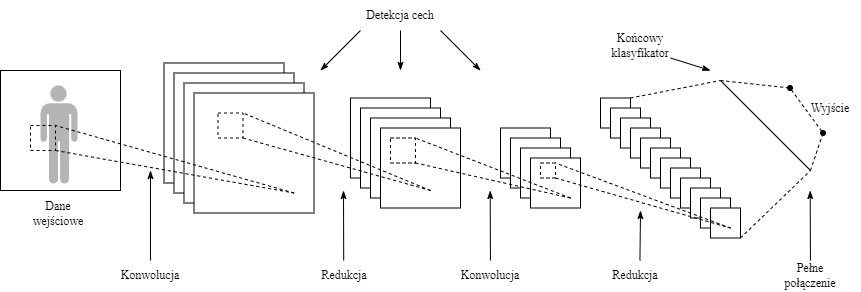
\includegraphics[width=\linewidth]{Obrazy/Rozdzial02/struktura.png}
    \caption{Schemat poglądowy architektury konwolucyjnej sieci neuronowej wykorzystującej \textit{pooling}.}
    \label{fig:struktura}
\end{figure}

\noindent
Wspomagając się rysunkiem \ref{fig:struktura}, można wyróżnić

\begin{enumerate}
    \item \textbf{warstwę wejściową}, reprezentującą obraz wejściowy do sieci. W zależności od rodzaju obrazu różni się ilość kanałów wejściowych wprowadzanych do pierwszej ukrytej warstwy, trzy kanały RGB w przypadku obrazów kolorowych lub jeden dla obrazów monochromatycznych,
    
    \item \textbf{warstwy konwolucyjne}, będące miejscem wykonywania konwolucji. W nich odbywa się  proces filtracji liniowej obrazu poprzez przesuwanie po obrazie maski jądra. Jako wynik operacji otrzymywana jest mapa cech.
        
        \begin{figure}[H]
        \centering
        \subfloat[Nałożenie maski nad wybraną część obrazu.]{\label{msk1}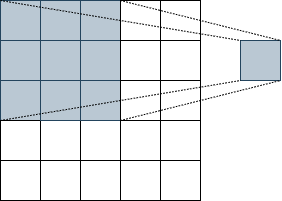
\includegraphics[width=.4\linewidth]{Obrazy/Rozdzial02/konwolucyja1.png}}
        \hspace{0.5cm}
        \subfloat[Powstawanie kolejnych pikseli po przesunięciu maski.]{\label{msk2}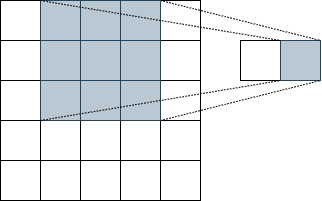
\includegraphics[width=.46\linewidth]{Obrazy/Rozdzial02/konwolucyja2.png}}\hfill
        \caption{Przesunięcie jądra maski 3x3 o krok konwolucji równy 1.}
        \label{fig:test}
        \end{figure}
        
        Przystępując do tworzenia warstwy konwolucyjnej konieczne jest zdefiniowanie i wybór odpowiednich parametrów 
        \begin{itemize}
            \item[--] rozmiar jądra (ang. \textit{kernel}), inaczej rozmiar filtra, który przesuwany będzie nad obrazem     wejściowym,
            \item[--] krok konwolucji (ang. \textit{stride}), który określa o ile pikseli na raz okno filtra zostanie     przesunięte,
            \item[--] rodzaj wypełnienia (ang. \textit{padding}) obramowania obrazu, aby zachować jednakowe wymiary     wejścia i wyjścia,
            \item[--] rodzaj funkcji aktywacji, odpowiadającej za wprowadzenie nieliniowości.
        \end{itemize}
    
    
    \item \textbf{warstwę redukującą} (ang. \textit{pooling)}, której celem jest zmniejszenie złożoności kolejnych warstw, tym samym zmniejszając liczby parametrów przekazywanych dalej i złożoność obliczeniową modelu. Wspomaga ona przeciwdziałanie przeuczeniu sieci.
        \begin{figure}[H]
            \centering
            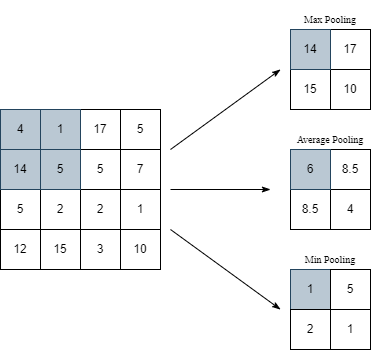
\includegraphics[width=0.5\linewidth]{Obrazy/Rozdzial02/pooling.png}
            \caption{Porównanie trzech typów puli.}
            \label{fig:pooling}
        \end{figure}

        Tak jak przedstawiono na rysunku \ref{fig:pooling} istnieją różne wersje \textit{poolingu}. Wykorzystując podany przykład z maską 2x2 i kroku konwolucji równemu 2 możemy mapować znajdujące się pod nią piksele na jeden jako
        \begin{itemize}
            \item[--] max pooling -  maksymalna wartość wszystkich pikseli,
            \item[--] average pooling - średnia wartość wszystkich pikseli,
            \item[--] min pooling - minimalna wartość wszystkich pikseli.
        \end{itemize}
        
    \item \textbf{warstwę w pełni połączoną}, zazwyczaj ostatnią warstwą sieci, w której wykonane są wszystkie możliwe połączenia między znajdującymi się w niej neuronami, a wyjściami poprzedniej warstwy. 
\end{enumerate}


% \hspace{0.4cm}
% Poza hiperparametrami potrzebnymi do stworzenia warstwy konwolucyjnej
% Rozpoczynając uczenie sieci konwolucyjnej konieczne jest dobranie jej hiperparametrów, do których należą

% \begin{itemize}
%     \item[--] liczba warstw konwolucyjnych ukrytych
%     \item[--] wymiar filtru, będący zazwyczaj maską kwadratową
%     \it
%     \item[--] krok przesunięcia maski tj. \textit{stride}
%     \item[--] 
% \end{itemize}
% \label{roz2.3}